\documentclass[10pt,t,aspectratio=169]{beamer}
%\usetheme{Berkeley}
\usepackage{graphicx}
\usepackage{amsmath}
\usepackage[american]{circuitikz}

% Packages to plot functions
\usepackage{pgfplots}
\pgfplotsset{compat=newest}

\usepackage{multicol}
\usepackage{multirow}
\usepackage{textcomp} % to use \textmu
\usepackage[absolute,overlay]{textpos} % to place floating text boxes with \begin{textblock*}{width}(x,y)
\usepackage{tcolorbox}
\usepackage{colortbl} % allows coloring cells of a table with \cellcolor{blue!25}

\title{Clase 1}
\subtitle{Semiconductores intrínsecos}
\author{Dr.-Ing. Juan José Montero Rodríguez}
\subject{Elementos Activos}
\institute{Escuela de Ingeniería Electrónica}
\date{Semestre II-2023}
\titlegraphic{
\includegraphics[height=12mm]{./figures/logoTEC.pdf}}


\begin{document}


\begin{frame}[t]
\titlepage
\end{frame}

\begin{frame}[t]
\frametitle{Elementos Pasivos y Activos}

\begin{columns}
  \begin{column}[t]{0.7\textwidth}
    \textbf{Elementos pasivos:}

    \begin{itemize}
        \item Dispositivos lineales.
        \item No controlan el flujo de corriente.
    \end{itemize}

    \vspace{3mm}
    \scalebox{0.9}{
    \begin{columns}
      \begin{column}[t]{2cm}
        \centering
        \textbf{Resistencia}
        %
        \[ i(t) = \dfrac{v(t)}{R} \]
        %
        \begin{circuitikz} \draw (0,0) to[R] (2,0); \end{circuitikz}
      \end{column}
      \begin{column}[t]{2cm}
        \centering
        \textbf{Capacitancia}
        %
        \[ i(t) = C \cdot \dfrac{dv(t)}{dt} \]
        %
        \begin{circuitikz} \draw (0,0) to[C] (2,0); \end{circuitikz}
      \end{column}
      \begin{column}[t]{3cm}
        \centering
        \textbf{Inductancia}
        %
        \[ i(t) = \dfrac{1}{L} \int_0^t v(t) dt + i(t_0) \]
        %
        \begin{circuitikz} \draw (0,0) to[L] (2,0); \end{circuitikz}
      \end{column}
    \end{columns}
    }

    \vspace{3mm}
    \begin{itemize}
      \item Tienen una característica de transferencia simétrica: funcionan igual ante tensiones positivas o negativas.
      \item Conducen en ambas direcciones.
      \end{itemize}
  \end{column}
  \begin{column}[t]{0.3\textwidth}
    \begin{figure}[H]
      \centering
      \pgfplotsset{width=\textwidth,compat=1.9}
      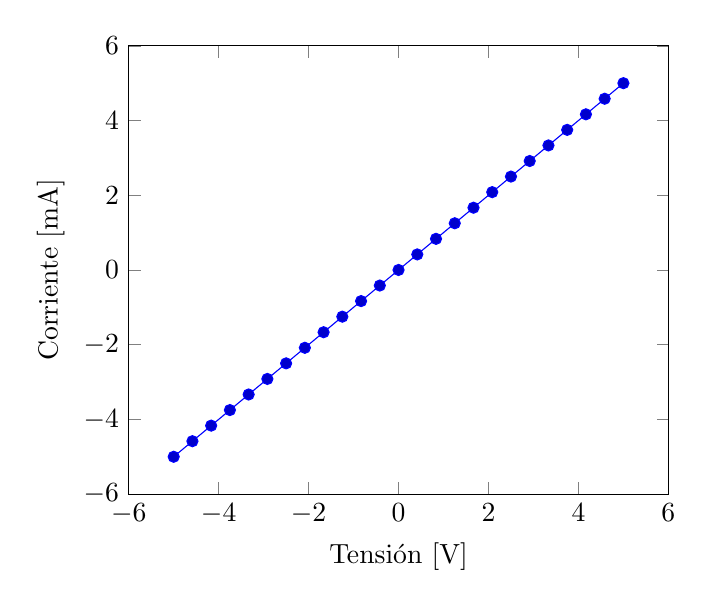
\begin{tikzpicture}[scale = 1]
        \begin{axis}[ 
          xlabel={Tensión [V]},
          ylabel={Corriente [mA]}
        ] 
          \addplot{x}; 
        \end{axis}
      \end{tikzpicture}
      \small{Característica de transferencia de una resistencia.}
      \end{figure}
    \end{column}
  \end{columns}
\end{frame}

\begin{frame}{Elementos Activos}

  \begin{columns}
    \begin{column}[t]{0.7\textwidth}
    \textbf{Elementos activos:}
    
    \begin{itemize}
        \item Dispositivos no lineales
        \item Conducción controlada por tensión
        \item Amplificación, rectificación, regulación
    \end{itemize}

    \vspace{3mm}
    \scalebox{0.9}{
    \begin{columns}
      \begin{column}[t]{2cm}
        \centering
        \textbf{Diodo}
        
        \[ i(t) \propto A(e^{V(t)/K} - 1) \]
        
        \begin{circuitikz} \draw (0,0) to[D] (2,0); \end{circuitikz}
        
        Exponencial
      \end{column}
      \begin{column}[t]{2cm}
        \centering
        \textbf{BJT}
        
        \[ i(t) \propto A(e^{V(t)/K} - 1) \]
        
        \begin{circuitikz} \draw (0,0) node[npn]{}; \end{circuitikz}
        
        Exponencial
      \end{column}
      \begin{column}[t]{3cm}
        \centering
        \textbf{MOSFET}
        
        \[ i(t) \propto A(V(t)-K)^2 \]
        
        \begin{circuitikz}[arrowmos] \draw (0,0) node[nmos]{}; \end{circuitikz}
        
        Cuadrática
      \end{column}
    \end{columns}
    }
  \end{column}
  \begin{column}[t]{0.3\textwidth}
    \begin{figure}[H]
      \centering
      \pgfplotsset{width=\textwidth,compat=1.9}
      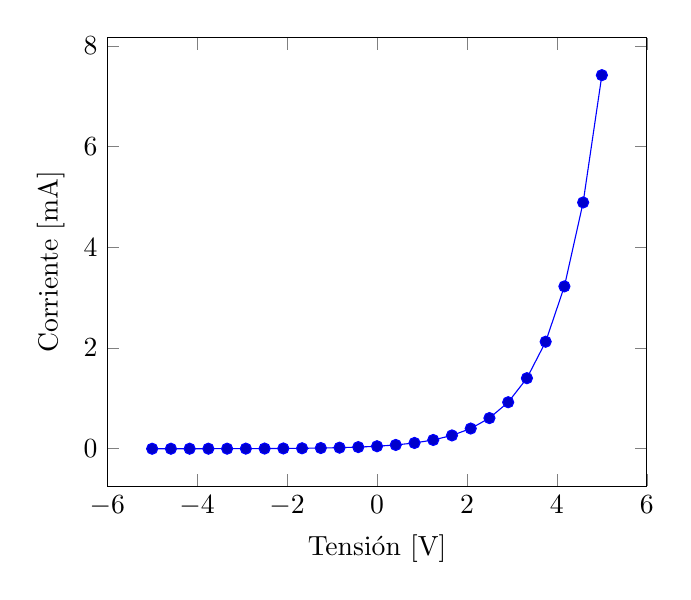
\begin{tikzpicture}[scale = 1]
          \begin{axis}[ 
            xlabel={Tensión [V]},
            ylabel={Corriente [mA]}
          ] 
            \addplot{0.05*e^x}; 
          \end{axis}
      \end{tikzpicture}
      \small{Característica de transferencia de un diodo.}
    \end{figure}
  \end{column}
\end{columns}
\end{frame}


\begin{frame}[t]
\frametitle{Clasificación de los Elementos}

Los elementos se agrupan de acuerdo a las propiedades metálicas como metales, no metales o semiconductores (metaloides).

\begin{figure}[H]
    \centering
    \begin{tabular}{ccccccc}
        I   & II  & III & IV  & V   & VI  & VII \\
        \cellcolor{blue!25} Li  & \cellcolor{blue!25} Be  & \cellcolor{red!25} B   & \cellcolor{green!25} C   & \cellcolor{green!25} N   & \cellcolor{green!25} O   & \cellcolor{green!25} F   \\
        \cellcolor{blue!25} Na  & \cellcolor{blue!25} Mg  & \cellcolor{blue!25} Al  & \cellcolor{red!25} Si  & \cellcolor{green!25} P   & \cellcolor{green!25} S   & \cellcolor{green!25} Cl  \\
        \cellcolor{blue!25}K   & \cellcolor{blue!25}Ca  & \cellcolor{blue!25}Ga  & \cellcolor{red!25} Ge  & \cellcolor{red!25} As  & \cellcolor{green!25} Se  & \cellcolor{green!25} Br  \\
    \end{tabular}

    \vspace{3mm}
    \begin{tabular}{ccc}
      \cellcolor{blue!25}Metales & \cellcolor{red!25}Semiconductores & \cellcolor{green!25}No metales \\
    \end{tabular}
\end{figure}

\textbf{Metales:} conductividad alta ($\sigma > 10^{6}$  S/m)

\vspace{2mm}
\textbf{Semiconductores:} conductividad intermedia ($10^{-6}$ S/m $< \sigma < 10^{-2}$ S/m)

\begin{itemize}
  \item Semiconductores elementales: Si, Ge
  \item Compuestos binarios: GaAs
  \item Compuestos ternarios: AlGaAs
  \item Compuestos cuaternarios: InGaAsP
\end{itemize}

\vspace{2mm}
\textbf{No metales:} conductividad baja ($\sigma < 10^{-9}$ S/m)
\end{frame}


\begin{frame}[t]
\frametitle{Sólidos Amorfos, Cristalinos y Policristalinos}

Los materiales se clasifican según su ordenamiento atómico en:

\begin{figure}[H]
  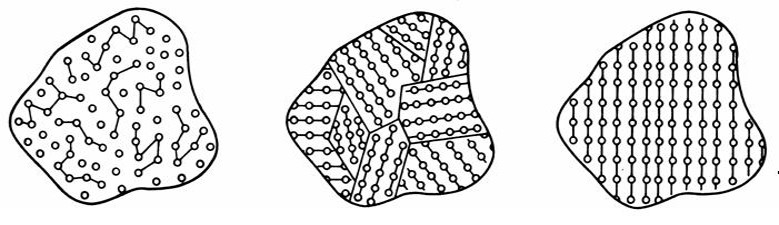
\includegraphics[width=12cm]{./figures/cristalinidad.jpg}
  \begin{columns}
    \begin{column}[t]{3.6cm}
      \centering
      \textbf{Amorfos}

      Átomos no siguen ningún orden, no forman estructura ordenada regular.
    \end{column}
    \begin{column}[t]{3.6cm}
      \centering
      \textbf{Policristalinos}

      Segmentos cristalinos, no estructura regular en todo el  material.
    \end{column}
    \begin{column}[t]{3.6cm}
      \centering
      \textbf{Cristalinos}

      Átomos forman una estructura regular en todo el material.
    \end{column}
  \end{columns}
\end{figure}
\end{frame}


\begin{frame}[t]
  \frametitle{Semiconductores Cristalinos}
  
  \begin{columns}
  
    \begin{column}{0.75\textwidth}
    
      Semiconductores utilizados principalmente en estado cristalino
      
      \begin{itemize}
        \item Materiales ultrapuros
        \item Ordenamiento regular de átomos en todo el cristal
      \end{itemize}
      
      \vspace{3mm}
      Silicio:
      
      \begin{itemize}
        \item Semiconductor dominante en microelectrónica
        \item Abundancia (28\% del peso de la corteza terrestre)
        \item Posibilidad de obtención de material de alta pureza
        \item 99.9999999\% para silicio de grado semiconductor
        \item Excelentes propiedades aislantes de SiO\textsubscript{2}
        \end{itemize}
        
    \end{column}
    
    \begin{column}{0.25\textwidth}
    
      \centering
      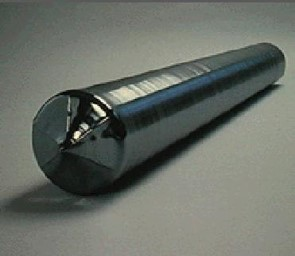
\includegraphics[width=\textwidth]{./figures/lingote.jpg}

      \small{Lingote de silicio}
      
      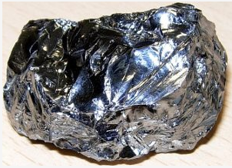
\includegraphics[width=\textwidth]{./figures/silicio-puro.png}

      \small{Silicio en estado natural}
      
    \end{column}
    
  \end{columns}
  
\end{frame}

\begin{frame}[t]
  \frametitle{Fabricación de Lingotes de Silicio}
  \begin{columns}
    \begin{column}[t]{0.5\textwidth}
      \centering
      \textbf{Método de Czochralski}

      \vspace{2mm}
      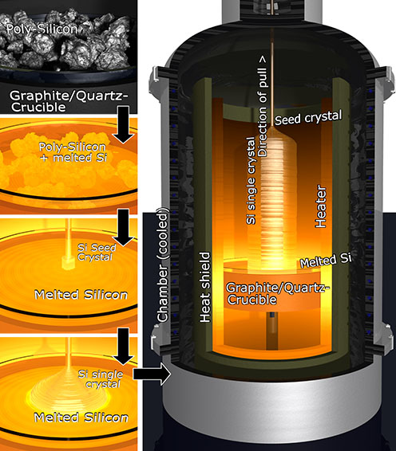
\includegraphics[height=6cm]{./figures/czochralski.png}
    \end{column}
    \begin{column}[t]{0.5\textwidth}
      \centering
      \textbf{Método de Zona Flotante}

      \vspace{2mm}
      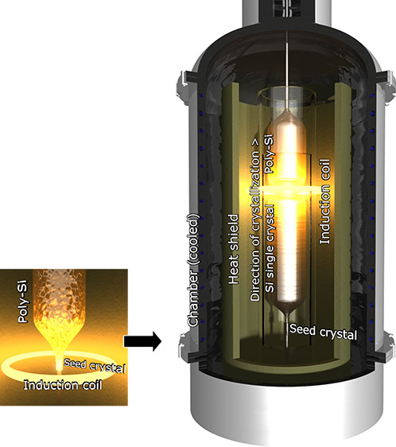
\includegraphics[height=6cm]{./figures/floatingzone.png}
    \end{column}
  \end{columns}

  \vspace{2mm}
  \centering
  \small{Referencia: Microchemicals GmbH}
\end{frame}


\begin{frame}[t]
  \frametitle{Celdas Unitarias}
  La celda unitaria es una porción del cristal que puede ser utilizada para replicar la totalidad del cristal original completo.
  \begin{itemize}
    \item No son necesariamente únicas: para un mismo cristal pueden existir distintas celdas unitarias con diferentes geometrías.
    \item Celda unitaria primitiva: la mínima celda unitaria posible.
  \end{itemize}

  \begin{columns}
    \begin{column}[t]{0.5\textwidth}
      \centering
      \textbf{En dos dimensiones:}
      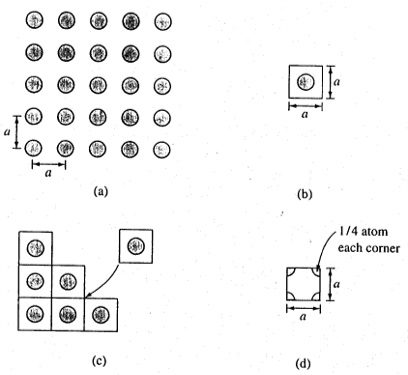
\includegraphics[width=5cm]{./figures/unitcell2d.png}
    \end{column}
    \begin{column}[t]{0.5\textwidth}
      \centering
      \textbf{En tres dimensiones:}
      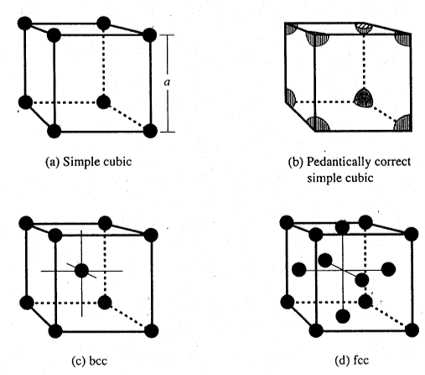
\includegraphics[width=5cm]{./figures/unitcell3d.png}
    \end{column}
  \end{columns}
\end{frame}


\begin{frame}
  \frametitle{Celda Unitaria del Silicio}

  \begin{itemize}
    \item El silicio presenta una estructura de tipo fcc (face centered cubic).
    \item Para los semiconductores mostrados, hay 8 átomos por celda unitaria.
  \end{itemize}
  
  \centering
  \vspace{3mm}
  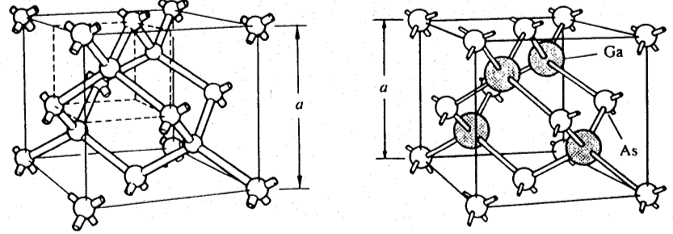
\includegraphics[width=12cm]{./figures/unitcell-silicon.png}

  \vspace{3mm}
  \begin{columns}
    \begin{column}[]{0.4\textwidth}
      \centering
      Estructura cristalina del diamante (silicio, germanio)
    \end{column}
    \begin{column}[]{0.4\textwidth}
      \centering
      Estructura cristalina de zinc blenda (zinc blende) (GaAs, ZnS)
    \end{column}
  \end{columns}

\end{frame}


\begin{frame}
  \frametitle{Planos Cristalinos en Silicio}
  
  La orientación del cristal afecta:

  \begin{itemize}
    \item Proceso de fabricación de circuitos integrados.
    \item Comportamiento de los dispositivos fabricados.
  \end{itemize}

  \vspace{3mm}
  Notación: Índices de Miller

  \vspace{5mm}
  \centering
  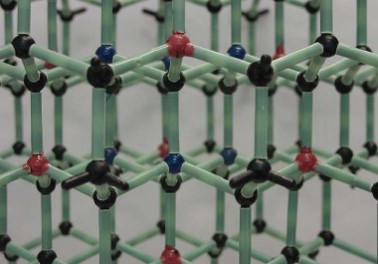
\includegraphics[height=0.2\textwidth]{./figures/silicon111.jpg}
  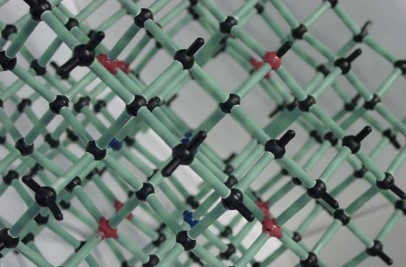
\includegraphics[height=0.2\textwidth]{./figures/silicon100.jpg}
  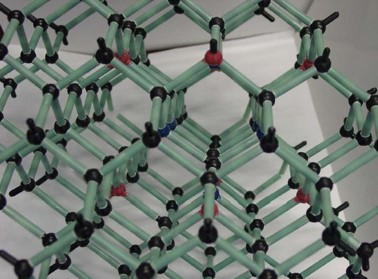
\includegraphics[height=0.2\textwidth]{./figures/silicon110.jpg}

  \begin{columns}
    \begin{column}[t]{3.5cm}
      \centering Plano (111)
    \end{column}
    \begin{column}[t]{3.5cm}
      \centering Plano (100)
    \end{column}
    \begin{column}[t]{3.5cm}
      \centering Plano (110)
    \end{column}
  \end{columns}
\end{frame}


\begin{frame}[t]
  \frametitle{Índices de Miller}

  \begin{columns}
  
    \begin{column}{0.65\textwidth}
    
      Pasos para determinar los índices:

      \begin{enumerate}
        \item Anotar el punto donde el plano interseca cada uno de los ejes.
        \item Tomar el recíproco de cada intersección.
        \item Eliminar las fracciones multiplicando por un número entero.
        \item Escribir el resultado en orden xyz, colocando entre paréntesis.
        \item Los números negativos se escriben con una línea sobre el número.
      \end{enumerate}
      
    \end{column}
    
    \begin{column}{0.35\textwidth}
    
      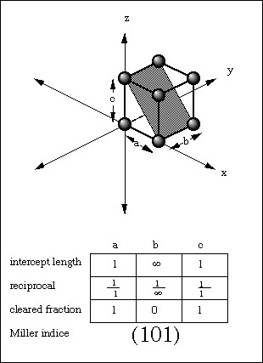
\includegraphics[width=\textwidth]{./figures/miller101.jpg}
      
    \end{column}
    
  \end{columns}
  
\end{frame}


\begin{frame}[t]
  \frametitle{Índices de Miller}

  \centering
  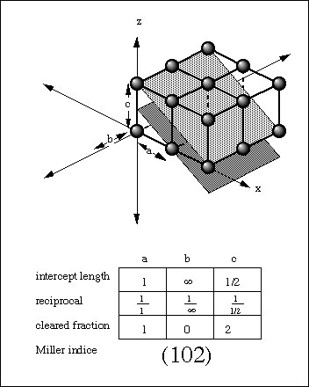
\includegraphics[height=7cm]{./figures/miller102.jpg}
  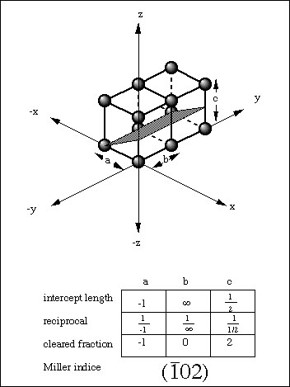
\includegraphics[height=7cm]{./figures/millern102.jpg}
\end{frame}


\begin{frame}[t]
  \frametitle{El Átomo de Hidrógeno}

  \begin{columns}
  
    \begin{column}{0.6\textwidth}
    
      El átomo de hidrógeno tiene un electrón y un protón
      
      \begin{itemize}
        \item El electrón orbita alrededor del núcleo con niveles de energía definidos
        \item Si el electrón pasa de un nivel a otro, absorbe energía o libera energía (medida en eV)
        \item $1\ eV = 1.602\times{}10^{-19}\ J$
      \end{itemize}

      \vspace{3mm}
      La energía está cuantizada:

      \[ E_H = -\dfrac{m_0 q^4}{2(4\pi{}\epsilon_0 \hbar \textbf{n})^2} = \dfrac{-13.6\ eV}{\textbf{n}^2} \]

      \centering
      \vspace{3mm}
      \textbf{n}=1, 2, 3, ...

      \flushleft
      \vspace{3mm}
      \textbf{Un electrón que se encuentra a una distancia infinita del núcleo posee una energía de cero (0 eV).}
    
    \end{column}
    
    \begin{column}{0.4\textwidth}
    
      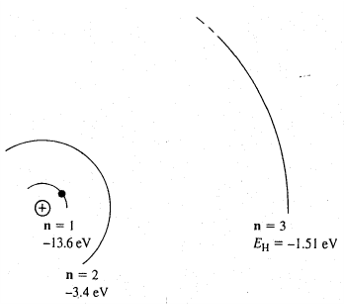
\includegraphics[width=\textwidth]{./figures/atom-hydrogen.png}
      
    \end{column}
    
  \end{columns}
  
\end{frame}


\begin{frame}[t]
  \frametitle{El Átomo de Silicio}

  \begin{columns}
  
    \begin{column}{0.6\textwidth}
    
      El átomo de silicio tiene 14 electrones
      
      \begin{itemize}
        \item 10 permanecen fuertemente ligados al núcleo
        \item 4 electrones externos se denominan electrones de valencia
      \end{itemize}

      \vspace{3mm}
      La configuración electrónica es: 1s\textsuperscript{2}2s\textsuperscript{2}2p\textsuperscript{6}3s\textsuperscript{2}3p\textsuperscript{2}

      \vspace{3mm}
      No puede haber dos electrones con el mismo nivel de energía (principio de exclusión de Pauli)
      
    \end{column}
    
    \begin{column}{0.4\textwidth}
    
      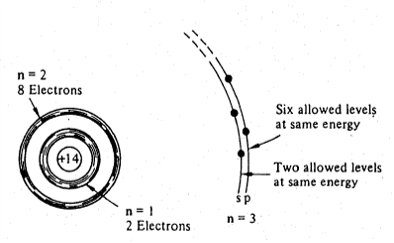
\includegraphics[width=\textwidth]{./figures/atom-silicon.png}
      
    \end{column}
    
  \end{columns}
  
\end{frame}


\begin{frame}[t]
  \frametitle{Modelo de Enlaces}

  \begin{columns}
  
    \begin{column}{0.5\textwidth}
    
      Describe los átomos y enlaces
      
      \begin{itemize}
        \item Círculo: átomo
        \item Línea: enlace covalente
      \end{itemize}

      \vspace{3mm}
      Cada átomo Si tiene 4 enlaces
      \begin{itemize}
        \item Se cumple regla del octeto
        \item Cuatro electrones propios
        \item Cuatro electrones compartidos
      \end{itemize}

      \vspace{3mm}
      \fbox{
      \begin{minipage}{6cm}
        \textbf{A una temperatura T = 0 K, \\ todos los electrones forman enlaces}
      \end{minipage}
      }
      
    \end{column}
    
    \begin{column}{0.5\textwidth}
    
      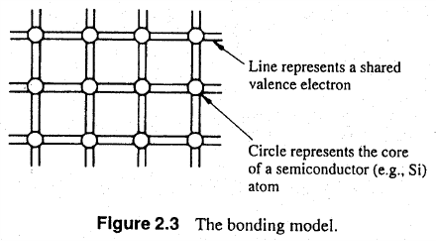
\includegraphics[width=\textwidth]{./figures/modelo-enlaces.png}
      
    \end{column}
    
  \end{columns}
  
\end{frame}


\begin{frame}[t]
  \frametitle{Modelo de Enlaces: Defectos en el Cristal}

  El modelo de enlaces permite describir defectos en la estructura cristalina.

  \centering
  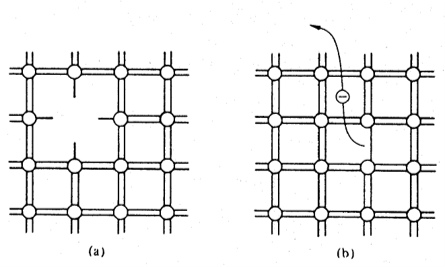
\includegraphics[width=0.6\textwidth]{./figures/modelo-defectos.png}

  \begin{columns}

    \begin{column}{0.20\textwidth}

    \end{column}
  
    \begin{column}{0.30\textwidth}
    
    \centering
    Átomo faltante
      
    \end{column}
    
    \begin{column}{0.30\textwidth}
    
      \centering
      Enlace roto
    \end{column}

    \begin{column}{0.20\textwidth}

    \end{column}
    
  \end{columns}

  \vspace{3mm}
  La limitación del modelo de enlaces es que no indica las energías de los electrones.
\end{frame}


\begin{frame}[t]
  \frametitle{Generación Térmica de Portadores de Carga}

  \begin{columns}
  
    \begin{column}{0.85\textwidth}
    
      Sobre los electrones:
      
      \begin{itemize}
        \item En estado de equilibrio a $T=0\ K$, todos los electrones del silicio forman enlaces con sus cuatro vecinos más cercanos.
        \item Cuando se eleva la temperatura, algunos enlaces se rompen. El electrón queda libre para moverse por todo el cristal. Este proceso se conoce como \textbf{generación}.
        \item La carga del electrón es $\boxed{q=-1.602\times{}10^{-19}\ C}$
      \end{itemize}

      Sobre los huecos:
      
      \begin{itemize}
        \item El electrón liberado deja un espacio vacío en el cristal, conocido como hueco.
        \item Otro electrón puede llegar a ocupar la posición del hueco, restaurando el enlace. Este proceso se conoce como \textbf{recombinación}.
        \item Los huecos pueden moverse por todo el cristal.
        \item La carga del hueco es $\boxed{q=+1.602\times{}10^{-19}\ C}$
      \end{itemize}
      
    \end{column}
    
    \begin{column}{0.15\textwidth}
    
      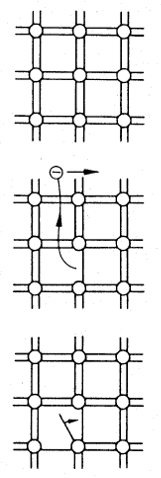
\includegraphics[width=\textwidth]{./figures/generacion.png}
    \end{column}
    
  \end{columns}
  
\end{frame}


\begin{frame}[t]
  \frametitle{El Concepto de Hueco}

  \begin{columns}
  
    \begin{column}[]{0.6\textwidth}
    
      El concepto de hueco es una representación de un enlace roto.

      \begin{itemize}
        \item Enlace roto representado por una partícula de carga positiva, con igual magnitud de carga que el electrón.
        \item Electrones y huecos interactúan en el proceso de conducción de corriente de huecos, por lo que se denominan portadores de carga.
        \item Conforme los electrones se mueven a la izquierda para llenar un hueco, el hueco se mueve a la derecha $\Rightarrow$ equivale a una corriente de huecos. 
        \item La corriente de huecos tiene la misma dirección que la corriente técnica
      \end{itemize}
      
    \end{column}
    
    \begin{column}[]{0.4\textwidth}
    
      \centering
      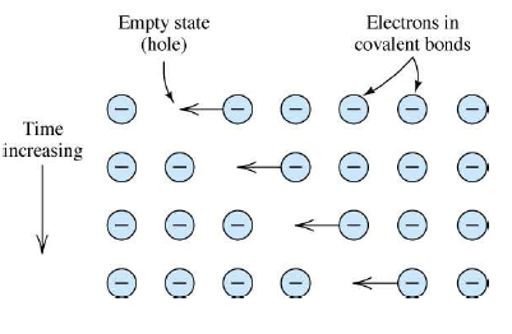
\includegraphics[width=\textwidth]{./figures/corriente-huecos.png}
      
    \end{column}
    
  \end{columns}
  
\end{frame}


\begin{frame}[t]
  \frametitle{Masa Efectiva de los Portadores de Carga}

  \begin{columns}
  
    \begin{column}[]{0.8\textwidth}
    
      \begin{itemize}
        \item Si se aplica un campo eléctrico $\mathcal{E}$ uniforme en el vacío, un electrón se mueve como consecuencia de una fuerza:
        \[ F = -q\mathcal{E} = m_0 \dfrac{dv}{dt} \]
        donde $m_0$ es la masa del electrón en el vacío ($m_0=9.1\times{}10^{-31}\ kg$).
      \end{itemize}
      
    \end{column}
    
    \begin{column}[]{0.2\textwidth}
    
      \centering
      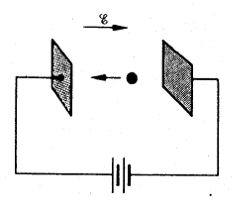
\includegraphics[width=\textwidth]{./figures/fuerza.png}
      
    \end{column}
    
  \end{columns}

  \vspace{3mm}
  \begin{columns}
  
    \begin{column}[]{0.8\textwidth}
    
      \begin{itemize}
        \item Para electrones en sólidos, la fuerza no se puede calcular tan fácilmente:
        \begin{itemize}
          \item Fuerzas electrostáticas con otros electrones
          \item Colisiones de electrones con el cristal
        \end{itemize}
        \item Se define la masa efectiva del electrón:
        \[ F = -q\mathcal{E} = m_n^* \dfrac{dv}{dt} \]
        donde $m_n^*$ es la masa efectiva del electrón ($m_n^*/m_0=1.18$ en silicio).
      \end{itemize}
      
    \end{column}
    
    \begin{column}[]{0.2\textwidth}
    
      \centering
      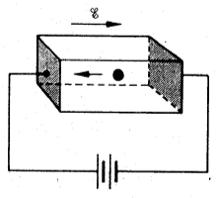
\includegraphics[width=\textwidth]{./figures/fuerza2.png}
      
    \end{column}
    
  \end{columns}
  
\end{frame}


\begin{frame}[t]
  \frametitle{Masa Efectiva de los Portadores de Carga}

  Lo mismo sucede con los huecos:

  \begin{itemize}
    \item Un hueco se desplaza libremente a través del cristal.
    \item El hueco experimenta una ``fuerza'' debido al campo eléctrico.
    \item El hueco es una ``partícula'' que también tiene masa efectiva.
  \end{itemize}

  \vspace{3mm}
La masa efectiva para electrones y huecos en distintos materiales:

\begin{table}[H]
  \centering
  \begin{tabular}{ccc}
  \hline \textbf{Material} & $m_n^*/m_0$ & $m_p^*/m_0$ \\
  \hline Si & 1.18 & 0.81 \\
  Ge & 0.55 & 0.36 \\
  GaAs & 0.066 & 0.52 \\
  \hline
\end{tabular}
\end{table}

Donde $m_0$ sigue siendo la masa del electrón en el vacío:

\[ m_0=9.1\times{}10^{-31}\ kg \]
\end{frame}


\begin{frame}[t]
  \frametitle{Concentración Intrínseca de Portadores de Carga}

  \begin{columns}
  
    \begin{column}[]{0.55\textwidth}
    
      La concentración de portadores en el silicio intrínseco (sin dopar) es:

      \[ n_i = 2 \left( \dfrac{2\pi{}m_n^* k T}{h^2} \right)^{3/2} \cdot{} e^{\dfrac{-E_g}{2kT}}\]

      Donde:

      \begin{itemize}
        \item $m_n^*$: masa efectiva del electrón
        \item $k$: constante de Boltzmann ($1.38\times{}10^{-23}\ J/K = 8.617\times{}10^{-5}\ eV/K$)
        \item $T$: temperatura en Kelvin
        \item $E_g$: Energía de la banda prohibida (1.12 eV para Silicio)
      \end{itemize}
      
      Nota: $1\ J = 1\ kg\cdot{}m^2/s^2$

    \end{column}
    
    \begin{column}[]{0.45\textwidth}
    
      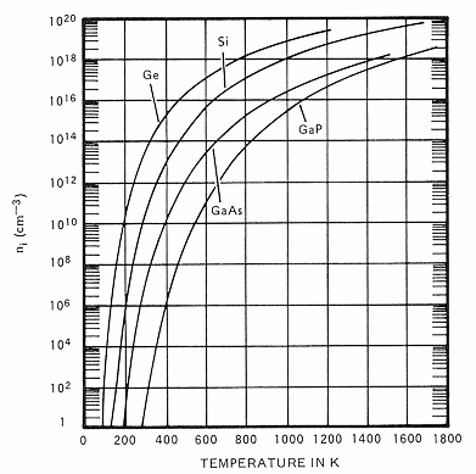
\includegraphics[width=\textwidth]{./figures/intrinsic-carrier-concentration.jpg}
      
    \end{column}
    
  \end{columns}
  
\end{frame}


\begin{frame}[t]
  \frametitle{Ejemplo: Concentración Intrínseca de Portadores de Carga}

  Calcule la concentración intrínseca de portadores para el silicio (Eg=1.12 eV) para una temperatura de 300 K.
  %
  \[ n_i = 2 \left( \dfrac{2\pi{}m_n^* k T}{h^2} \right)^{3/2} \cdot{} e^{\dfrac{-E_g}{2kT}}\]
  %
  \small \[ n_i = 2 \left( \dfrac{2\pi{} (1.18\times{}9.1\times{}10^{-31}\ kg) (1.38\times{}10^{-23}\ J/K) (300\ K)}{(6.626\times{}10^{-34}\ J\cdot{}s)^2} \right)^{3/2} \cdot{} e^{\dfrac{-1.12\ eV}{2(8.617\times{}10^{-5}\ eV/K)(300\ K))}}\]
  %
  \normalsize \[ n_i = (3.2095\times{}10^{25}) \left[ \dfrac{kg\ kg\ m^2\ K\ s^2}{m^4\ kg^2\ s^2\ K} \right]^{3/2} \cdot (3.9089\times{}10^{-10}) \]
  %
  \[ n_i = (1.2546\times{}10^{16}) \left[ \dfrac{1}{m^2} \right]^{3/2} = (1.2546\times{}10^{16}) \left[ \dfrac{1}{m^{6/2}} \right] \]
  %
  \[ n_i = (1.2546\times{}10^{16}) \left[ \dfrac{1}{m^{3}} \right] \times{} \dfrac{(1\ m)^3}{(100\ cm)^3} = 1.2546\times{}10^{10}\ cm^{-3} \approx \boxed{10^{10}\ cm^{-3}} \]

\end{frame}


\begin{frame}[t]
  \frametitle{Ejemplo: Cantidad de Átomos Si en 1 cm\textsuperscript{3}}

  Para el silicio en estado intrínseco, la densidad es $2.33\ g/cm^3$, la masa molar es $28.09\ g/mol$ y el número de Avogadro es $6.02\times{}10^{23}\ atomos/mol$. Calcule:

  \begin{itemize}
    \item La cantidad de átomos de silicio que hay en un trozo de 1 cm\textsuperscript{3}.
    \[ 2.33\dfrac{g}{cm^3} \times{}  \dfrac{1\ mol}{28.09\ g} \times{} \dfrac{6.02\times{}10^{23}\ atomos}{1\ mol} = 4.99\times{}10^{22}\ atomos/cm^{3} \]
    \item La cantidad de enlaces existentes en ese trozo de silicio de 1 cm\textsuperscript{3}.
    \[ 4.99\times{}10^{22}\ \dfrac{atomos}{cm^3} \times{} \dfrac{4\ enlaces}{1\ atomo} = 1.996\times{}10^{23}\ enlaces/cm^3 \]
    \item La razón de enlaces totales en comparación con enlaces rotos, a 
    temperatura ambiente.
    \[ \dfrac{1.996\times{}10^{23}\ enlaces\ completos/cm^3}{10^{10}\ enlaces\ rotos/cm^3} = 1.996\times{}10^{13} \]
  \end{itemize}
  
  Esto significa que hay un solo enlace roto (electrón libre) en $2\times{}10^{13}$ enlaces completos.

\end{frame}


\begin{frame}{Lecturas recomendadas}
    
\end{frame}

\end{document}
